\PassOptionsToPackage{unicode=true}{hyperref} % options for packages loaded elsewhere
\PassOptionsToPackage{hyphens}{url}
%
\documentclass[]{article}
\usepackage{lmodern}
\usepackage{amssymb,amsmath}
\usepackage{ifxetex,ifluatex}
\usepackage{fixltx2e} % provides \textsubscript
\ifnum 0\ifxetex 1\fi\ifluatex 1\fi=0 % if pdftex
  \usepackage[T1]{fontenc}
  \usepackage[utf8]{inputenc}
  \usepackage{textcomp} % provides euro and other symbols
\else % if luatex or xelatex
  \usepackage{unicode-math}
  \defaultfontfeatures{Ligatures=TeX,Scale=MatchLowercase}
\fi
% use upquote if available, for straight quotes in verbatim environments
\IfFileExists{upquote.sty}{\usepackage{upquote}}{}
% use microtype if available
\IfFileExists{microtype.sty}{%
\usepackage[]{microtype}
\UseMicrotypeSet[protrusion]{basicmath} % disable protrusion for tt fonts
}{}
\IfFileExists{parskip.sty}{%
\usepackage{parskip}
}{% else
\setlength{\parindent}{0pt}
\setlength{\parskip}{6pt plus 2pt minus 1pt}
}
\usepackage{hyperref}
\hypersetup{
            pdftitle={STA212 : Devoir : aspects pratiques},
            pdfauthor={Eltarr, Durand},
            pdfborder={0 0 0},
            breaklinks=true}
\urlstyle{same}  % don't use monospace font for urls
\usepackage[margin=1in]{geometry}
\usepackage{color}
\usepackage{fancyvrb}
\newcommand{\VerbBar}{|}
\newcommand{\VERB}{\Verb[commandchars=\\\{\}]}
\DefineVerbatimEnvironment{Highlighting}{Verbatim}{commandchars=\\\{\}}
% Add ',fontsize=\small' for more characters per line
\usepackage{framed}
\definecolor{shadecolor}{RGB}{248,248,248}
\newenvironment{Shaded}{\begin{snugshade}}{\end{snugshade}}
\newcommand{\AlertTok}[1]{\textcolor[rgb]{0.94,0.16,0.16}{#1}}
\newcommand{\AnnotationTok}[1]{\textcolor[rgb]{0.56,0.35,0.01}{\textbf{\textit{#1}}}}
\newcommand{\AttributeTok}[1]{\textcolor[rgb]{0.77,0.63,0.00}{#1}}
\newcommand{\BaseNTok}[1]{\textcolor[rgb]{0.00,0.00,0.81}{#1}}
\newcommand{\BuiltInTok}[1]{#1}
\newcommand{\CharTok}[1]{\textcolor[rgb]{0.31,0.60,0.02}{#1}}
\newcommand{\CommentTok}[1]{\textcolor[rgb]{0.56,0.35,0.01}{\textit{#1}}}
\newcommand{\CommentVarTok}[1]{\textcolor[rgb]{0.56,0.35,0.01}{\textbf{\textit{#1}}}}
\newcommand{\ConstantTok}[1]{\textcolor[rgb]{0.00,0.00,0.00}{#1}}
\newcommand{\ControlFlowTok}[1]{\textcolor[rgb]{0.13,0.29,0.53}{\textbf{#1}}}
\newcommand{\DataTypeTok}[1]{\textcolor[rgb]{0.13,0.29,0.53}{#1}}
\newcommand{\DecValTok}[1]{\textcolor[rgb]{0.00,0.00,0.81}{#1}}
\newcommand{\DocumentationTok}[1]{\textcolor[rgb]{0.56,0.35,0.01}{\textbf{\textit{#1}}}}
\newcommand{\ErrorTok}[1]{\textcolor[rgb]{0.64,0.00,0.00}{\textbf{#1}}}
\newcommand{\ExtensionTok}[1]{#1}
\newcommand{\FloatTok}[1]{\textcolor[rgb]{0.00,0.00,0.81}{#1}}
\newcommand{\FunctionTok}[1]{\textcolor[rgb]{0.00,0.00,0.00}{#1}}
\newcommand{\ImportTok}[1]{#1}
\newcommand{\InformationTok}[1]{\textcolor[rgb]{0.56,0.35,0.01}{\textbf{\textit{#1}}}}
\newcommand{\KeywordTok}[1]{\textcolor[rgb]{0.13,0.29,0.53}{\textbf{#1}}}
\newcommand{\NormalTok}[1]{#1}
\newcommand{\OperatorTok}[1]{\textcolor[rgb]{0.81,0.36,0.00}{\textbf{#1}}}
\newcommand{\OtherTok}[1]{\textcolor[rgb]{0.56,0.35,0.01}{#1}}
\newcommand{\PreprocessorTok}[1]{\textcolor[rgb]{0.56,0.35,0.01}{\textit{#1}}}
\newcommand{\RegionMarkerTok}[1]{#1}
\newcommand{\SpecialCharTok}[1]{\textcolor[rgb]{0.00,0.00,0.00}{#1}}
\newcommand{\SpecialStringTok}[1]{\textcolor[rgb]{0.31,0.60,0.02}{#1}}
\newcommand{\StringTok}[1]{\textcolor[rgb]{0.31,0.60,0.02}{#1}}
\newcommand{\VariableTok}[1]{\textcolor[rgb]{0.00,0.00,0.00}{#1}}
\newcommand{\VerbatimStringTok}[1]{\textcolor[rgb]{0.31,0.60,0.02}{#1}}
\newcommand{\WarningTok}[1]{\textcolor[rgb]{0.56,0.35,0.01}{\textbf{\textit{#1}}}}
\usepackage{graphicx,grffile}
\makeatletter
\def\maxwidth{\ifdim\Gin@nat@width>\linewidth\linewidth\else\Gin@nat@width\fi}
\def\maxheight{\ifdim\Gin@nat@height>\textheight\textheight\else\Gin@nat@height\fi}
\makeatother
% Scale images if necessary, so that they will not overflow the page
% margins by default, and it is still possible to overwrite the defaults
% using explicit options in \includegraphics[width, height, ...]{}
\setkeys{Gin}{width=\maxwidth,height=\maxheight,keepaspectratio}
\setlength{\emergencystretch}{3em}  % prevent overfull lines
\providecommand{\tightlist}{%
  \setlength{\itemsep}{0pt}\setlength{\parskip}{0pt}}
\setcounter{secnumdepth}{0}
% Redefines (sub)paragraphs to behave more like sections
\ifx\paragraph\undefined\else
\let\oldparagraph\paragraph
\renewcommand{\paragraph}[1]{\oldparagraph{#1}\mbox{}}
\fi
\ifx\subparagraph\undefined\else
\let\oldsubparagraph\subparagraph
\renewcommand{\subparagraph}[1]{\oldsubparagraph{#1}\mbox{}}
\fi

% set default figure placement to htbp
\makeatletter
\def\fps@figure{htbp}
\makeatother


\title{STA212 : Devoir : aspects pratiques}
\author{Eltarr, Durand}
\date{09/05/2020}

\begin{document}
\maketitle

\hypertarget{arbre-de-duxe9cision-unique}{%
\section{Arbre de décision unique}\label{arbre-de-duxe9cision-unique}}

\begin{Shaded}
\begin{Highlighting}[]
\KeywordTok{setwd}\NormalTok{(}\StringTok{'/home/lokmen/Documents/ENSTA/STAT/STA212/STA212DM'}\NormalTok{)}
\KeywordTok{rm}\NormalTok{(}\DataTypeTok{list =} \KeywordTok{objects}\NormalTok{())}
\KeywordTok{graphics.off}\NormalTok{()}
\NormalTok{OJ=}\KeywordTok{read.csv}\NormalTok{(}\StringTok{"oj.csv"}\NormalTok{, }\DataTypeTok{header =} \OtherTok{TRUE}\NormalTok{)}
\CommentTok{#View(OJ)}
\end{Highlighting}
\end{Shaded}

On regarde la nature de nos données. On a 1070 observations pour 18
variables différentes. Les variables categorielles sont
\(\texttt{Purchase}\) qui admet deux niveaux, et \(\texttt{Store 7}\)
qui admet aussi deux niveaux. Les autres sont numériques.

\begin{Shaded}
\begin{Highlighting}[]
\KeywordTok{str}\NormalTok{(OJ) }
\end{Highlighting}
\end{Shaded}

\begin{verbatim}
## 'data.frame':    1070 obs. of  18 variables:
##  $ Purchase      : Factor w/ 2 levels "CH","MM": 1 1 1 2 1 1 1 1 1 1 ...
##  $ WeekofPurchase: int  237 239 245 227 228 230 232 234 235 238 ...
##  $ StoreID       : int  1 1 1 1 7 7 7 7 7 7 ...
##  $ PriceCH       : num  1.75 1.75 1.86 1.69 1.69 1.69 1.69 1.75 1.75 1.75 ...
##  $ PriceMM       : num  1.99 1.99 2.09 1.69 1.69 1.99 1.99 1.99 1.99 1.99 ...
##  $ DiscCH        : num  0 0 0.17 0 0 0 0 0 0 0 ...
##  $ DiscMM        : num  0 0.3 0 0 0 0 0.4 0.4 0.4 0.4 ...
##  $ SpecialCH     : int  0 0 0 0 0 0 1 1 0 0 ...
##  $ SpecialMM     : int  0 1 0 0 0 1 1 0 0 0 ...
##  $ LoyalCH       : num  0.5 0.6 0.68 0.4 0.957 ...
##  $ SalePriceMM   : num  1.99 1.69 2.09 1.69 1.69 1.99 1.59 1.59 1.59 1.59 ...
##  $ SalePriceCH   : num  1.75 1.75 1.69 1.69 1.69 1.69 1.69 1.75 1.75 1.75 ...
##  $ PriceDiff     : num  0.24 -0.06 0.4 0 0 0.3 -0.1 -0.16 -0.16 -0.16 ...
##  $ Store7        : Factor w/ 2 levels "No","Yes": 1 1 1 1 2 2 2 2 2 2 ...
##  $ PctDiscMM     : num  0 0.151 0 0 0 ...
##  $ PctDiscCH     : num  0 0 0.0914 0 0 ...
##  $ ListPriceDiff : num  0.24 0.24 0.23 0 0 0.3 0.3 0.24 0.24 0.24 ...
##  $ STORE         : int  1 1 1 1 0 0 0 0 0 0 ...
\end{verbatim}

\hypertarget{analyse-univariuxe9e-et-bivariuxe9e}{%
\subsection{Analyse Univariée et
Bivariée}\label{analyse-univariuxe9e-et-bivariuxe9e}}

On procéde à une analyse univariée des variables. On se sert de la
description des variables ainsi que des commandes \(\texttt{summary}\),
\(\texttt{plot}\) et \(\texttt{table}\).

Par exemple, on peut voir que les variables \(\texttt{SpecialCH}\) et
\(\texttt{SpecialMM}\) prennent seulement les valeurs 0 et 1.

\begin{Shaded}
\begin{Highlighting}[]
\KeywordTok{table}\NormalTok{(OJ}\OperatorTok{$}\NormalTok{SpecialCH)}
\end{Highlighting}
\end{Shaded}

\begin{verbatim}
## 
##   0   1 
## 912 158
\end{verbatim}

\begin{Shaded}
\begin{Highlighting}[]
\KeywordTok{plot}\NormalTok{(OJ}\OperatorTok{$}\NormalTok{SpecialCH)}
\end{Highlighting}
\end{Shaded}

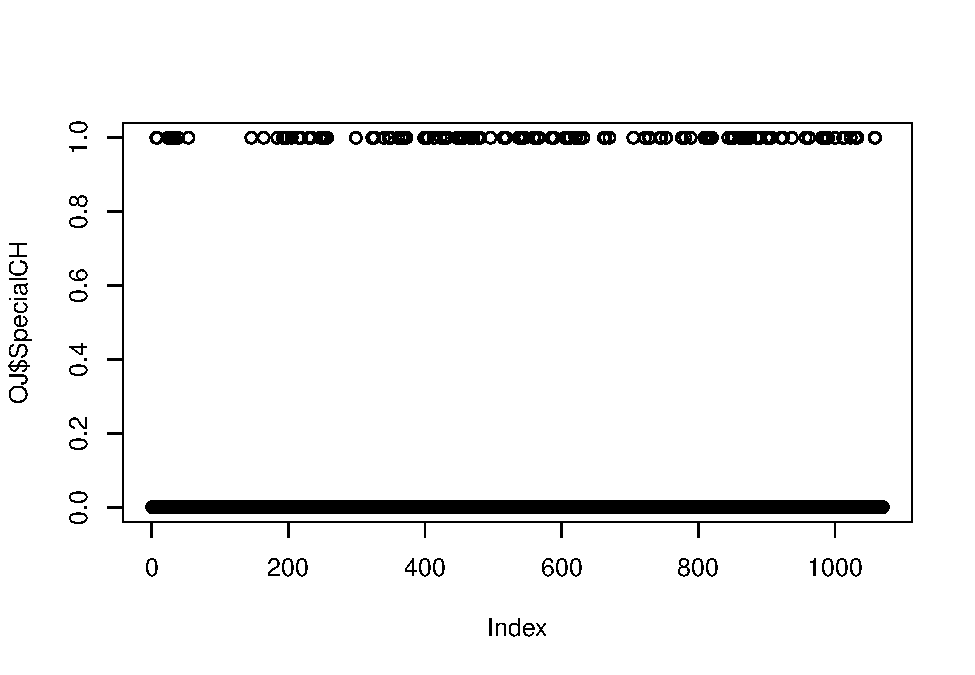
\includegraphics{durand_eltarr_files/figure-latex/unnamed-chunk-3-1.pdf}

\begin{Shaded}
\begin{Highlighting}[]
\KeywordTok{table}\NormalTok{(OJ}\OperatorTok{$}\NormalTok{SpecialMM)}
\end{Highlighting}
\end{Shaded}

\begin{verbatim}
## 
##   0   1 
## 897 173
\end{verbatim}

\begin{Shaded}
\begin{Highlighting}[]
\KeywordTok{plot}\NormalTok{(OJ}\OperatorTok{$}\NormalTok{SpecialMM)}
\end{Highlighting}
\end{Shaded}

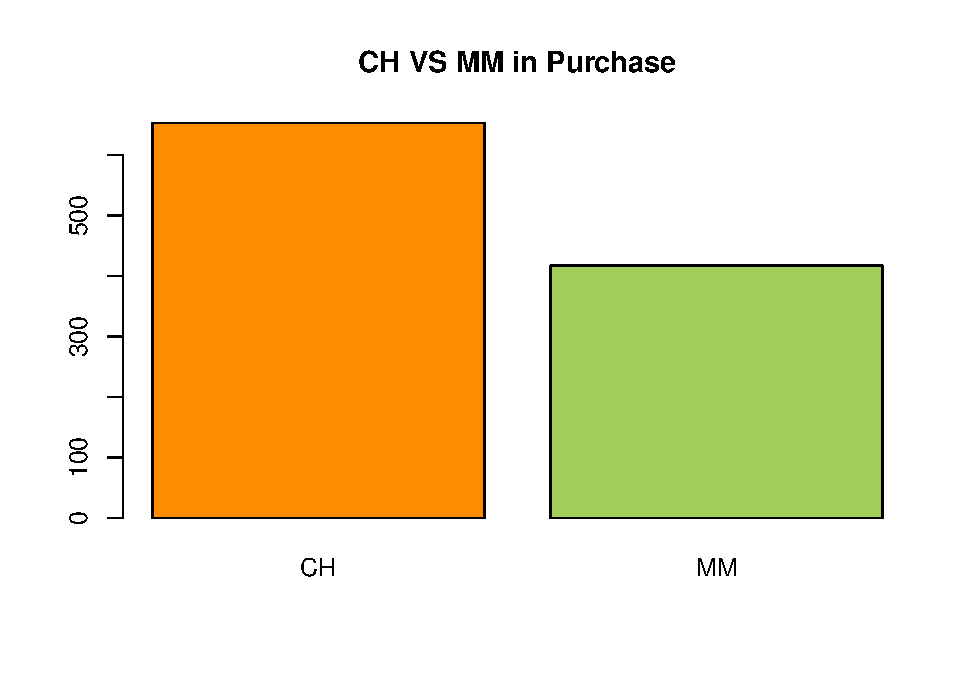
\includegraphics{durand_eltarr_files/figure-latex/unnamed-chunk-4-1.pdf}
De la même manière \(\texttt{STORE}\) ne prend que les valeurs entre 0
et 4.

\begin{Shaded}
\begin{Highlighting}[]
\KeywordTok{table}\NormalTok{(OJ}\OperatorTok{$}\NormalTok{STORE)}
\end{Highlighting}
\end{Shaded}

\begin{verbatim}
## 
##   0   1   2   3   4 
## 356 157 222 196 139
\end{verbatim}

\begin{Shaded}
\begin{Highlighting}[]
\KeywordTok{plot}\NormalTok{(OJ}\OperatorTok{$}\NormalTok{STORE)}
\end{Highlighting}
\end{Shaded}

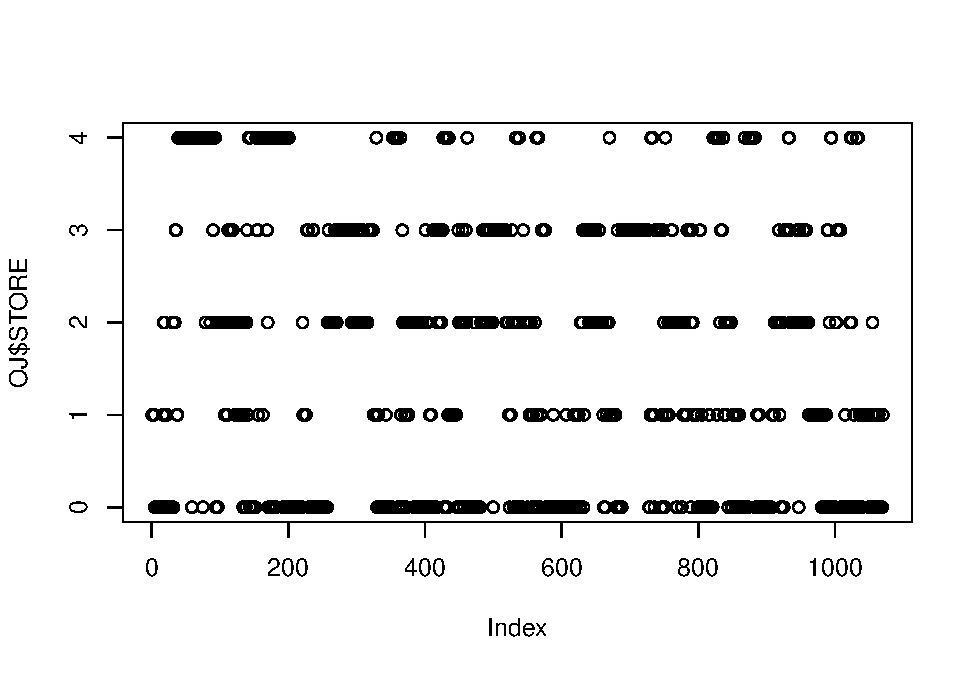
\includegraphics{durand_eltarr_files/figure-latex/unnamed-chunk-5-1.pdf}

On préfère alors les transformer en variables catégorielles:

\begin{Shaded}
\begin{Highlighting}[]
\NormalTok{OJ}\OperatorTok{$}\NormalTok{SpecialMM <-}\StringTok{ }\KeywordTok{as.factor}\NormalTok{(OJ}\OperatorTok{$}\NormalTok{SpecialMM)}
\NormalTok{OJ}\OperatorTok{$}\NormalTok{SpecialCH <-}\StringTok{ }\KeywordTok{as.factor}\NormalTok{(OJ}\OperatorTok{$}\NormalTok{SpecialCH)}
\NormalTok{OJ}\OperatorTok{$}\NormalTok{STORE <-}\StringTok{ }\KeywordTok{as.factor}\NormalTok{(OJ}\OperatorTok{$}\NormalTok{STORE}\OperatorTok{+}\DecValTok{1}\NormalTok{) }\CommentTok{## On préfère avoir des valeurs entre 1 et 5.}
\end{Highlighting}
\end{Shaded}

Ensuite, on voit que la variable \(\texttt{PriceDiff}\) est une
combinaison des deux variables \(\texttt{SalePriceMM}\) et
\(\texttt{SalePriceCH}\). On décide alors de la retrouver.

\begin{Shaded}
\begin{Highlighting}[]
\NormalTok{OJ <-}\StringTok{ }\KeywordTok{subset}\NormalTok{(OJ, }\DataTypeTok{select=}\OperatorTok{-}\NormalTok{PriceDiff)}
\KeywordTok{length}\NormalTok{(OJ)}
\end{Highlighting}
\end{Shaded}

\begin{verbatim}
## [1] 17
\end{verbatim}

\hypertarget{including-plots}{%
\subsection{Including Plots}\label{including-plots}}

You can also embed plots, for example:

\includegraphics{durand_eltarr_files/figure-latex/pressure-1.pdf}

Note that the \texttt{echo\ =\ FALSE} parameter was added to the code
chunk to prevent printing of the R code that generated the plot.

\end{document}
